\section{Registerallokation}


Die Registerallokation gehört zu den globalen Optimierungen. Sie hat zum Ziel,
möglichst viele der Variablen so lange wie möglich in den Prozessorregistern zu
halten. Hat man mehr Variablen zur selben Zeit als Register, muss man Werte
auslagern (spillen).


\subsection{Einfacher Top-Down Ansatz}

Die Register werden nach Anzahl Verwendungen der Variablen vergeben.

\textbf{Algorithmus}

\begin{enumerate}
	\item Lies das gesamte Programm (linear in Zeit) und bestimme, wie oft jede
		Variable verwendet wird. Jede Variable erhält eine Priorität gemäss der
		Häufigkeit ihres Auftretens.
	\item Sortiere die Variablen gemäss Prioritäten.
	\item Ordne den Variablen Register zu.
		\begin{itemize}
			\item Falls genug Register vorhanden sind: jede Variable bekommt ein
				Register.
			\item Sonst: verteile gemäss Priorität und reserviere Register für das
				Einlagern und Auslagern aus dem Memory.
		\end{itemize}
	\item Schreib den modifizierten Code wieder in eine Datei.
\end{enumerate}

\textbf{Vorteile}

\begin{itemize}
	\item Sehr einfach.
	\item Funktioniert, falls genug Register vorhanden sind.
\end{itemize}


\subsection{Einfacher Bottom-Up Ansatz}

Von unten nach oben versucht man einfach beim Auftreten einer Variable zu
bestimmen:

\begin{itemize}
	\item Ist die Variable in einem Register? Wenn ja: okay!
	\item Wenn nein: ist ein Register frei? Wenn ja: okay!
	\item Wenn nein: spill. Es wird die Variable ausgelagert, welche am längsten
		nicht mehr benötigt wird.
\end{itemize}


\subsection{Linear Scan}

\textbf{Algorithmus}

\begin{enumerate}
	\item Liveness-Analyse $\Rightarrow$ Liste mit Live Intervallen
	\item Sortiere gemäss Startpunkt der Live Intervalle.
	\item Intervall-Analyse:
	\begin{enumerate}
		\item Prüfe, ob Variablen nicht mehr benötigt werden. Falls ja: gib diese
			Register frei.
		\item Falls genügend Register vorhanden sind: weiterfahren (Register
			zuordnen). Falls zuwenig Register vorhanden sind: Spilling (beispielsweise
			jene Variablen, welche den spätesten Endpunkt haben).
	\end{enumerate}
\end{enumerate}

\hspace{15mm} \includegraphics[width=0.5\textwidth]{images/liveness}


\subsection{Register Interference Graph}
\label{subsec:rig}

Zwei temporäre Variablen, welche gleichzeitig lebendig sind, können nicht das
selbe Register belegen.

Register Interference Graph (RIG / IG):

\begin{itemize}
	\item Knoten repräsentieren (temporäre) Variablen.
	\item Kanten verbinden Knoten / Variablen, welche gleichzeitig lebendig sind.
	\item Zwei Variablen können das selbe Register belegen, falls sie keine
		verbindende Kante haben.
\end{itemize}

\textbf{Beispiel}

\begin{minipage}[t]{0.3\textwidth}\ttfamily
	\textrm{Live Sets:}\\\\
	\{b,c,f\}\\
	\{a,c,f\}\\
	\{c,d,f\}\\
	\{c,d,e,f\}\\
	\{c,e\}\\
	\{b,c,e,f\}\\
	\{c,f\}\\
	\{b\}
\end{minipage}%
%
\begin{minipage}[t]{0.5\textwidth}
	Graph:\\\\
	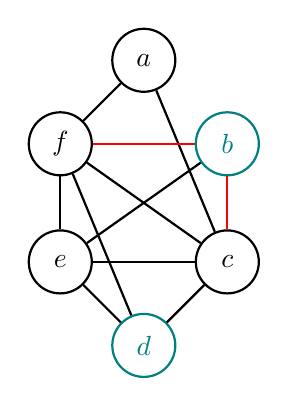
\begin{tikzpicture}[auto,node distance=1.5cm,thick]

		\tikzstyle{state}=[shape=circle,draw,minimum size=8mm]

		\node[state] (a) {$a$};
		\node[state] (b) [below right of=a, color=teal] {$b$};
		\node[state] (c) [below of=b] {$c$};
		\node[state] (d) [below left of=c, color=teal] {$d$};
		\node[state] (e) [above left of=d] {$e$};
		\node[state] (f) [below left of=a] {$f$};

		\path (a) edge (c)
					(a) edge (f)
					(b) edge [color=red] (c)
					(b) edge (e)
					(b) edge [color=red] (f)
					(c) edge (d)
					(c) edge (e)
					(c) edge (f)
					(d) edge (e)
					(d) edge (f)
					(e) edge (f);

	\end{tikzpicture}
\end{minipage}

Schlussfolgerung:

\begin{itemize}
	\item \texttt{\{b,c,f\}}: Die Variablen \texttt{b}, \texttt{f} und \texttt{c}
		können nicht im selben Register gespeichert werden.
	\item Die Variablen \texttt{b} und \texttt{d} können das selbe Register
		verwenden.
\end{itemize}


\subsection{Graph Coloring}

Graph Coloring ordnet den Knoten eines Graphen Farben zu. Benachbarte Knoten
müssen unterschiedliche Farbe haben. Ein Graph ist \texttt{k}-färbbar, falls er
mithilfe von \texttt{k} Farben gefärbt werden kann.

Das Problem des \hyperref[subsec:rig]{Register Interference Graphs} kann auf das
Graph Coloring Problem abgebildet werden. Dabei entsprechen die Farben den
Registern und \texttt{k} ist die Anzahl Maschinen-Register.

Falls der \hyperref[subsec:rig]{RIG} \texttt{k}-färbbar ist, dann existiert eine
Registerdarstellung mit nicht mehr als \texttt{k} Registern.

Das Graph Coloring Problem (und somit das Register Allocator Problem) ist
NP-Hart. Es gibt jedoch heuristische Lösungsverfahren, wie z.B. der Chaitin
Algorithmus.

Wenn der optimistische Chaitin Algorithmus schief geht, müssen wir Variablen
spillen. Auch für die Auswahl der auszulagernden Variablen gibt es nur
heuristische Ansätze.
